\documentclass[12pt]{article}

% Packages
\usepackage{graphicx}
\usepackage{amsmath}
\usepackage{amsfonts}
\usepackage{amssymb}
\usepackage[letterpaper,top=2cm,bottom=2cm,left=3cm,right=3cm,marginparwidth=1.75cm]{geometry}
\usepackage{minted}
\usepackage{rotating}
\usepackage{pdflscape}
\usepackage{csvsimple}
\usepackage{pgfplotstable}
\usepackage{multicol}
\usepackage{supertabular}
\usepackage{booktabs}
\usepackage{longtable}
\pgfplotsset{compat=newest}

\makeatletter
\let\mcnewpage=\newpage
\newcommand{\TrickSupertabularIntoMulticols}{%
\renewcommand\newpage{%
    \if@firstcolumn%
        \hrule width\linewidth height0pt%
            \columnbreak%
        \else%
          \mcnewpage%
        \fi%
}%
}
\makeatother



% Title page
\title{Hand in 2 \\ Information Theory}
\author{Fredrick Nilsson \\ fr2037ni-s}
\date{\today}

\begin{document}

\maketitle

\newpage

\section*{Report}

The file was successfully compressed from 152089 bytes to 87688 bytes.
The original file had an entropy of 4.568, and the average character length of the compressed text is 4.612,
this satisfies the optimal codeword length theorem \(H_D(X) \le L \le H_D(X) + 1\).
The huffman tree is shown in figure \ref{fig:tree}, while the codebook combined with the frequency table is shown in the codebook section.
The code for everything can be found in the source code section.

\begin{landscape}
    \begin{figure}
        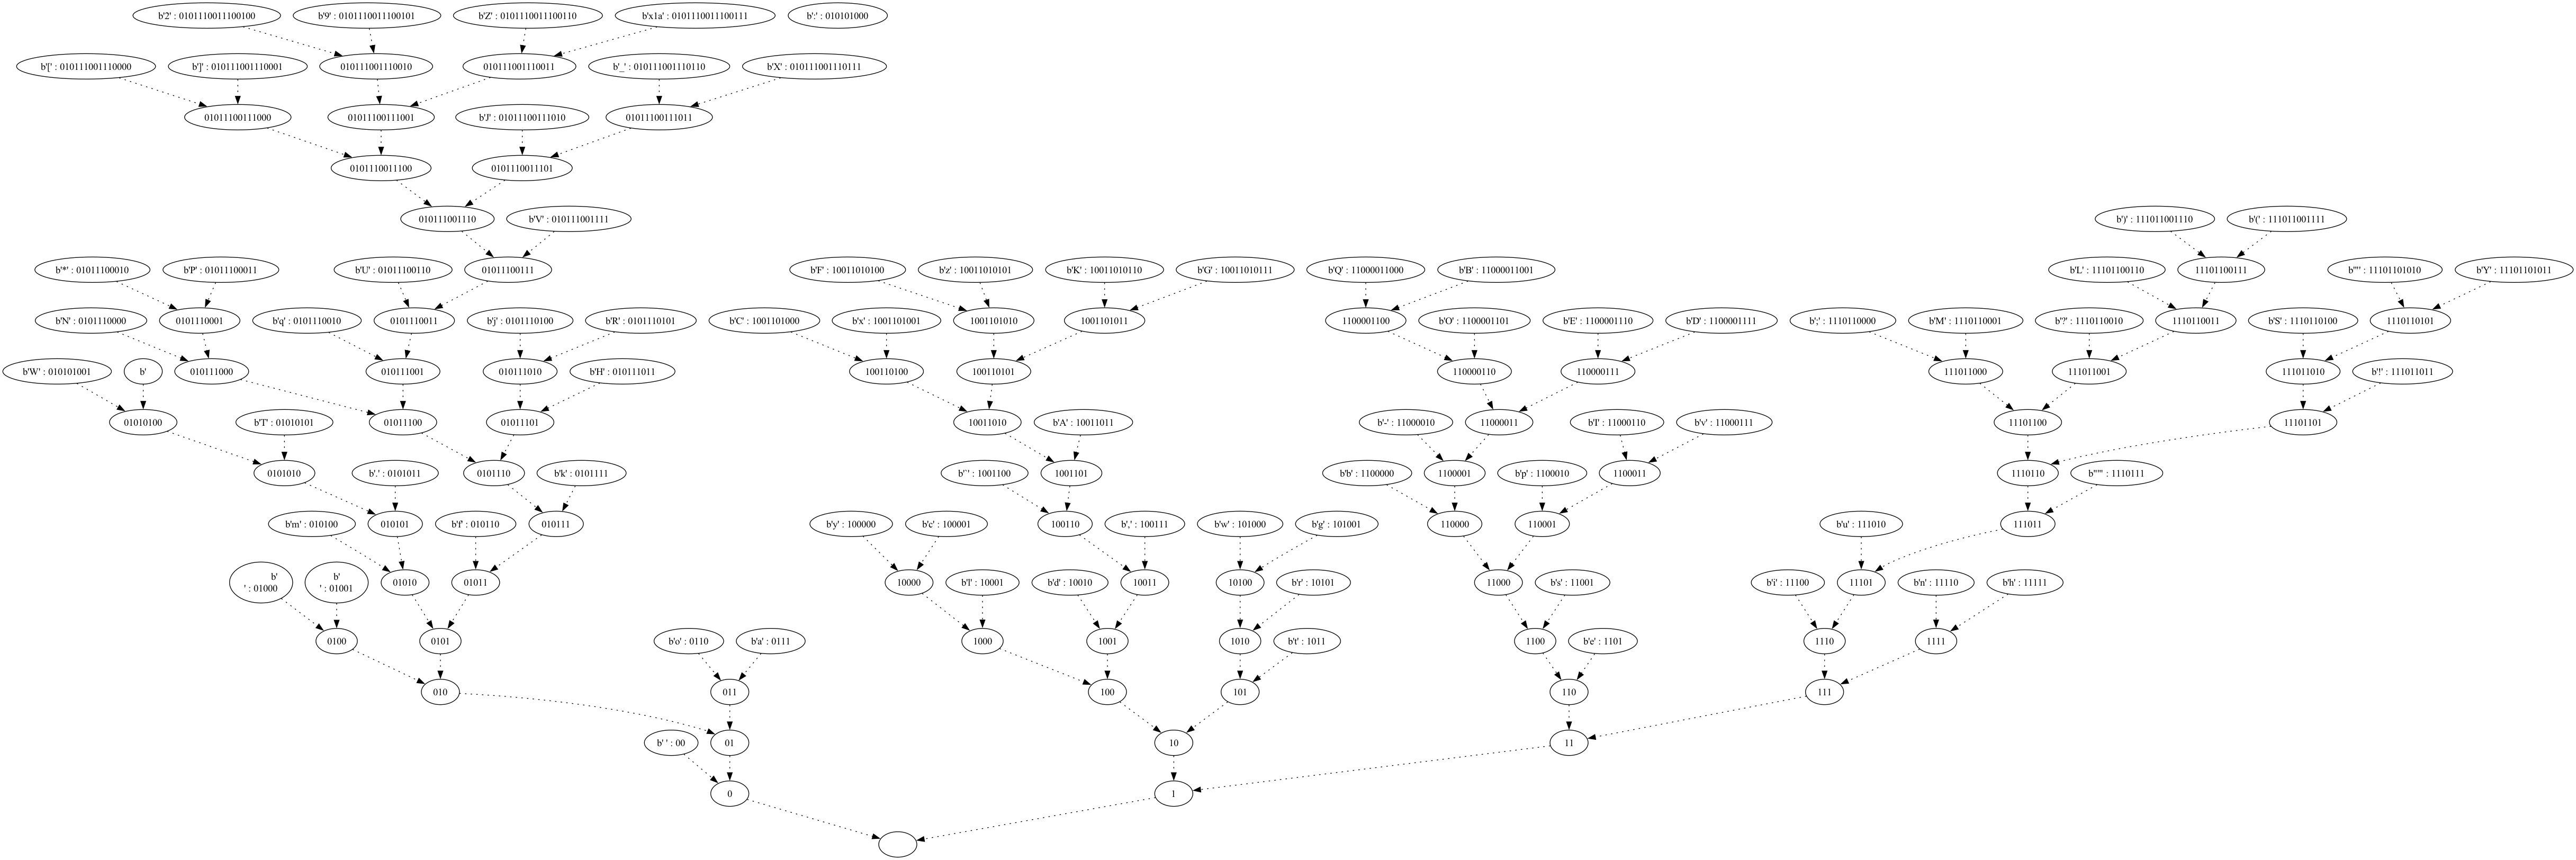
\includegraphics[width=1.6\textwidth]{../outputs/postorder_traversal.png}
        \caption{The huffman tree}
        \label{fig:tree}
    \end{figure}
\end{landscape}

\section*{Source code}
\inputminted[breaklines]{python}{../handin.py}

\newpage
\section*{Codebook}

\newbox\myb
\setbox\myb\vbox{\hsize=\dimexpr(\textwidth-\columnsep)/2\relax
\makeatletter
\chardef\LT@end@pen\z@
\makeatother
\begin{longtable}{lll}
    \toprule
    \textbf{Ascii} & \textbf{Count} & \textbf{Code}\\
    \midrule
    \endhead
    \bottomrule
    \endfoot
    \csvreader[
        late after line=\\,
        respect all,
        ]
    {../outputs/code_table.csv}{symbol=\symbol,probability=\probability,code=\code}{\symbol & \probability & \code}
\end{longtable}}
\begin{multicols*}{2}
\unvbox\myb
\end{multicols*}
\end{document}
